\documentclass[a4paper, twocolumn]{article}
\newcommand{\pversion}{0.5}
\newcommand{\papertitle}{NGI Use Cases: Smarter Workflow Processing in Climate/Weather}

\usepackage[a4paper, margin=2cm]{geometry}

\usepackage[utf8]{inputenc}
\usepackage[T1]{fontenc}
\usepackage{graphicx}
\usepackage[english]{babel}
\usepackage[colorlinks=true,urlcolor=red]{hyperref}
\usepackage{url}
\usepackage{cleveref}
\usepackage{todonotes}

\usepackage{multicol}
\setlength{\columnsep}{1cm}

\usepackage{fancyhdr}
\fancyhead{}
\fancyfoot{}
\fancyhead[l]{\papertitle~(Version: \pversion)}
\fancyhead[r]{
\includegraphics[height=1em]{ngi-logo}}
\fancyfoot[r]{\thepage}
\pagestyle{fancy}
\renewcommand{\headrulewidth}{1pt}
\renewcommand{\footrulewidth}{1pt}

\usepackage{titling}
\pretitle{\begin{center}\Large\bfseries}
\posttitle{\end{center}\vskip 0.5em}

\graphicspath{{./assets/}}

\title{\papertitle}

\author{Julian M. Kunkel
  \textit{University of Reading}
	\and
  Chris Hoffman
  \textit{National Center for Atmospheric Research}
}
\date{Version: \pversion; \today}


\begin{document}
\maketitle
\thispagestyle{fancy}

\section*{Abstract}
The efficient, convenient, and robust execution of data-driven workflows and enhanced data management are key for productivity in scientific computing and computer-aided Research, Development and Engineering (RD\&E).
As workflows become increasingly complex and blend beyond data centers while at the same time storage hierarchies becomes deeper, the community investigates means to re-organize storage access to fully utilize such environments.

In the NGI Forum, we believe workflows composed of data, compute and communication intensive tasks should drive the interfaces and hardware configurations to best support these programming models.
In this whitepaper, we describe how workflows for climate and weather could benefit from higher-level abstraction for data flows.
The document serves the purpose to motivate subsequent NGI activity, the implementation of described features will likely differ from the sketched solutions.

\section{Next Generation Workflows}
\label{sec:ngWorkflows}

This section illustrates how workflows could be run and optimized by smart runtime implementations.


\subsection{Climate/Weather in 2020+}

This workflow gives an idea how the climate and weather community could utilize emerging concepts in 2020+.
A generic overview of the workflows for climate and weather is given in \Cref{fig:climateWeather}.

Prediction of the weather in the near future (hours, known as nowcasting; days or weeks -- seasonal) is performed by executing workflows consisting of several processing steps. The execution of a workflow engine that orchestrates the individual execution steps is not explicitly included in the workflow description.

For weather prediction, these workflows are schedules on a regular basis, e.g., a prediction is performed every four hours.
The prediction is based on observational data and outputs data products that are processed further and distributed to customers.

\subsubsection{Execution of a weather workflow}



\begin{figure}[b]
  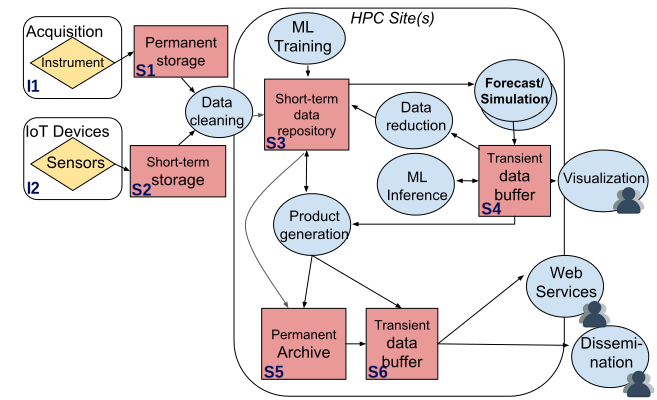
\includegraphics[width=\columnwidth]{climateweather-workflow}
  \caption{Future Climate and Weather Workflows}
  \label{fig:climateWeather}
\end{figure}


First, data sources providing up-to-date data (such as near-real-time satellite sources and weather stations, I1) are ingested into a local permanent repository (S1). These data may be supplemented by the increasing number of IoT and mobile sensor devices (I2) which data may be stored in a short-term storage (S2) with a limited life-time.
A weather service utilizing a HPC site ingests this data onto a local repository (S3). During this process, observational data is cleaned and reduced, e.g., by reducing resolution (subsampling).
An ensemble of forecasts (several parallel simulation applications) are started using a subset of the latest weather information -- typically each of the applications differs only in how the simulation is initialized.
They start with a warm up period using data from, e.g., 24 hours in the past. While a forecast runs it may use the data from I1/I2 to augment the simulated data with actual observations until the model time and the actual time matches and prediction of future weather starts.
While the ensemble of forecast runs, it computes various relevant output variables that may be stored in a transient data buffer (S4) and/or perform data transformation and analysis in-situ/in-transit. For example, a computed variables may be output, visualized and analyzed further by users even as the simulation continues. To identify patterns (events of interests for meteorologists), machine learning may be applied in the processing pipeline. Identified events may trigger further actions on the visualization, triggering additional data outputs, and controlling data reduction. To reduce the data volume for the ensemble, a data reduction selectively chooses data from the ensemble to preserve (on the repository S3, just before it is stored in the archive S5); this may be a typical run/minimum/maximum or runs that contain certain events as identified from the machine learning.
The generation of data products is either known beforehand, and calculated using a workflow during the ensemble run, or calculated post-mortem.
The former case is typical for weather applications. In the latter case, data products can be created offline from the stored output of the forecasts -- this allows users to request new or modified data products from the simulations via the web interface.
Machine learning can be applied in this workflow to identify relevant patterns in the data, supervised training involves the scientist selecting the phenomenon of interest presumably interactively using data visualization. The system should be able to quickly build a model and suggest other data with the similar phenomena to reduce the effort of the scientist to browse through all the data.

A selection of data products together are stored on a long-term (permanent) archive (S5).
Scientists over the world typically interact with web services to access data products on the long-term archive or to apply certain post-processing procedures to create new data products. This data is typically cached (S6) both at source before dissemination and by users in their workflow. When a new data product is requested it may actually trigger the recomputation of the data because it is cheaper than keeping all data products on a permanent storage.

Note that the box depicts “HPC-sites” that executes most parts of the workflow, however, not necessarily this must be a single data center. Scientists already work in a distributed fashion, downloading certain data products and performing subsequent data analysis locally, on other remote sites, data centers, or in the cloud. It is expected, thought, that the initial data production is kept on the site where the data is produced as the data volume is reduced significantly in this process.

\subsubsection{Execution of a climate workflow}

Generation of insight for a climate experiment differs from the weather case by several aspects: Firstly, the data (S2) from IOT devices (I2) is not used.
Secondly, in most cases scientists conduct new experiments, i.e., the result is a-prior unknown. Thus, a more exploratory and interactive use is expected.
For model intercomparison projects, once the variables and experiments to investigate are clear, a mass replication (execution) of the use case under different starting conditions takes place. These planned experiments come with less explorative nature, yet diagnosis of abnormal execution behavior may be investigated interactively.
Due to the vast amount of different experiments, the data management features of NGI are useful to simplify the data handling; for instance, by utilizing scientific metadata to specify the difference between different experiments differences between model output can be computed directly.


\subsection{Extreme Data Generation}

This section discusses a use case illustrating how the aforementioned concepts integrate into a smart system.
Consider the case in which a group of users conducts an experiment at large scale (a tightly coupled hero run on an HPC system) to gather new insight about small scale phenomenon.
This experiment generates raw data of a huge volume (e.g., several Petabytes on existing systems).
The user may know certain (diagnostic) post-processing that must be conducted on the data, but since the scientists work at the frontier of knowledge, it is usually unclear which features to look for and which data products to create.
Over a period of several month scientists will analyze a subset of data (e.g., two regions of 10 GiB each) potentially using machine learning to identify the further analysis steps that shall be conducted on the full dataset.
Once this is done, they register the analysis workflow and wait for all data products.

The user specifies the workflow defining the characteristics of the processing and the data and include that the final data product must be retained for 10 years.
The workflow also indicates that the data products are used in manual analysis and this may take several months.
Note that users do not deal with namespace issues but provide scientifically relevant metadata for the raw data and the data products.
At creation time of data products, these are semantically linked to the workflow and may be found when inspecting metadata for the created raw data.

\medskip

We envision the following support of the runtime for this use case:
The workflow description gives the scheduler various options; firstly, the final data product must be accessible for 10 years; it may decide that it is cost-efficient to store the data on a tape archive, a subset of the data region should be stored for in-depth analysis and likewise a low-resolution version of the should be created.
In another environment and depending on characteristics, the scheduler may have decided to not persist the huge data output but preserve a container for the application to allow recomputation -- but we will discuss the former case.

An I/O-enabled resource manager will dispatch the hero run exclusively once there is enough storage capacity available on the archive storage system such as tape and I/O bandwidth is available.
The system may schedule the post-processing, data reduction and subset creation, while  data transfer occurs in-transit on the client node or dedicated compute resources and picks a fast storage system for these products.
That means a data-driven streaming workflow is applied to minimize reading of data during the post-processing workflow.
The raw output is meanwhile directly stored on tape for archival purpose (e.g., as it must be kept for several years due to policies of the funding agency).
The sample data is a replicate of a subset of the raw data's domain and stored for inspection on a storage system supporting good random I/O workloads.
If a user inspects the metadata, one can see that fragments with a subset of data are stored on fast storage and the other parts on slow archival storage.
Once the user registers the final workflow, i.e., requests data processing on the full dataset, the system has to process the vast amount of data on tape.

Depending on the exact workflow, there are opportunities for the system:
Thanks to liquid computing, parts of the workflow can be executed directly on tape drives and the network thinning out the amount of data that needs to be transferred while reading.
Alternatively, we may retrieve the data from archive storage and create a copy on a faster storage system but -- since relevant parts of the workflow access pattern are known -- can reorganize the replicas of the fragment while data is fetched and, thus, optimize I/O for the subsequent accesses of the workflow.


\paragraph{In-Situ Analysis}

A user should be able any time to inspect and analyze data that is currently produced without changing the application code or even knowing a priori that this is an intent.
Let us extend the previous case of the hero run; now the user may decide to visually analyze a subset of data and a low-resolution output of the data while the data is generated.
We assume a node or visualization cluster has been allocated for this purpose.
An NGI enabled visualization tool would be able to query the metadata and search for the experiment currently conducted.
Then the region of interest is selected by the user.
In the best case, some derived data products could be reused but it is expected that the tool submits new tasks (code snippets for liquid computing) to the runtime to perform data analysis and reduction.
The system will create additional I/O streams and run the analysis codes in streaming mode as much as possible while it feeds the output to the application.
This would allow us to perform filter operations on the process creating the raw data.
If the volume of the produced data is too high, a workflow can be registered to create data products on the storage with good random I/O characteristics.
The visualization is then constantly updated according to the NGI semantics.

\section{Data Archival}
This scenario is a more conservative perspective utilizing NGI to replace data archival interfaces. 
This section is not meant to replace current archival systems, but instead of introduce capabilities that may not be present.
It also shows an incremental strategy to improve existing HPC environments.

\subsection{Introduction}
The archive strategy at many centers has been to have a large monolithic storage based system. 
These systems locked into vendor hardware and vendor software. 
There are typically minimal amount of additonal software that can be used with certain hardware. 
Features can be requested and implemented based on critical mass of user need or through non-recurring-engineering (NRE) funding. 
NRE is typically not available to many center besides the largest or the most well funded. 
HPC Centers may have a unique feature or capability that is wanted and while a request for enhancement is submitted, it may take a while to get critical mass, if at all.
Other features that may work with the underlying technology such as adding a new configuration or hardware component must be pre-approval from vendor before being integrated into the storage ecosystem.
This use case can work in a community driven model to add capabilities and features due to the FOSS nature.

Introduction of many physical tiers becomes troublesome for users to pre-migrate their data for usage or for archival purposes.
Physical tiers can be part of a namespace with many physical tiers into a single logical tier or an environment may have many logical tiers that are tied to their physical tier
This section will address ways to combine the many types of physical tiers into appropriate logical tiers, thus allows physical tiers have multiple uses.

The heterogeneous hierarchy of storage tiers have varying levels of performance and different economic models. 
For example, a burst buffer tier has been introduced for high IOPs and throughput to accelerate codes.
This tier is much smaller in capacity due to the cost of flash.
Various data retention boundaries may not align with an HPC storage system’s lifetime. 
This can be apparent when a storage system is years old and a new project spanning a decade.
Due to constantly changing use cases and generational technology shifts, a user may not be aware of proper use of a storage system.
For example, a user may store a data set in HPSS, which is commonly used for a long term archival solution.
This user then frequently recalls data from this solution.
A more optimized use case would be to use a near-line solution, such as Campaign Storage for warm active data sets.
In some cases, workflow may not be known until a project progresses.

Another unknown is future capabilities and layout of a storage system.
This storage system could introduce a new storage tier or combine multiple tiers into fewer logical tiers.
This also introduces significant effort in education, workflow optimization, and data stewardship.
This can cause extra effort of system administrators and users alike.
This future solution will address these challenges by giving a user more flexibility via workflow improvements.
We conclude that crucially in the HPC ecosystem, a middleware translation layer is needed which supports various backend storage solutions whether Commercial-off-the-shelf (COTS) solutions supplied or open source software (OSS).
This could be NGI.
A generic overview of this workflow is given in \Cref{fig:dataLifecycle}

\begin{figure}[b]
  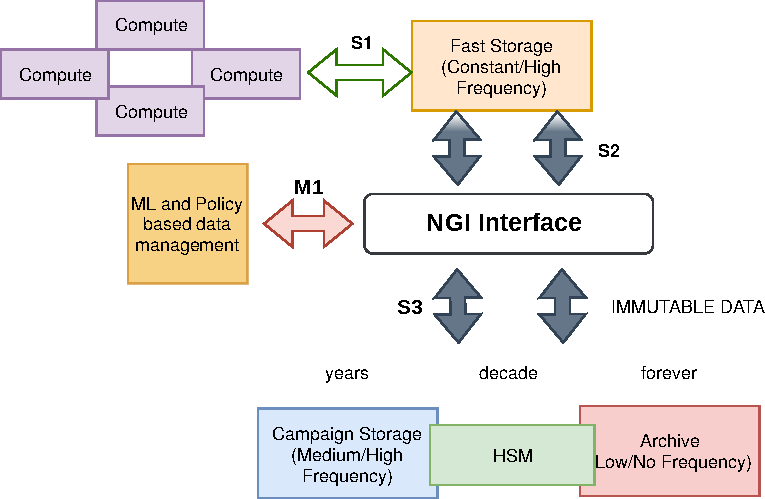
\includegraphics[width=0.75\columnwidth]{datalifecycle-workflow}
  \caption{Future Data Lifecycle Workflows}
  \label{fig:dataLifecycle}
\end{figure}

\subsubsection{Execution of the workflow}

First data sources are read and written from/to an HPC supercomputer.
(S1) shows I/O between a compute and primary data store, that may be POSIX or another interface.
This storage has high-performance characteristics for bandwidth, latency and I/O operations.
This data will be selected by the user for archival or migration off this location via a data movement tool (this is depicted in S2).
Instead of using proprietary interfaces, NGI could be used.
The respective tools translate on the fly from the native interface of one data store to the NGI interface.
NGI is in charge to make the decision how to layout the data on one or multiple storage backends (S3).
These backends are fully pluggable and customizable solutions.
Under the hood a backend -- such as tape -- may need additional Data Movers or File Transfer Agents (FTA) to perform the work efficiently; we will not discuss this further in this paper.
(M1) is the smart data management powered by Machine Learning that also takes user-defined migration policies and rules into account.
(M1) works with the data movers to migrate data back and forth without manual user intervention.
A user is able to read, write and delete immutable data and then allow for various data retention policies.


\paragraph{Optimized Data Placement}
The user will have to define the relevant properties of the data (such as how long that data shall be stored) and workflow and the system administrator provides the definition of the extensible storage landscape.
NGI will utilize machine learning techniques based on empirical data models for optimized management and placement of the data itself.
The result is to use each storage tier in the intended use case with minimal effort of user.
These storage tier can be tape or spinning disk media.

For example, assume a large dataset of hundreds of TiBs was put on a spinning disk archive (Campaign Storage), but only a specific variable with 10 GiB of data is accessed.
A potential operation would be that through data policies migrate other variables, that are unused, to a tape based system.
This will allow for more efficient uses of economics of storage media based on the temperature of the variables.
Another strategy would be to store the first timestep(s) on disk while storing the remainder on tape.
This allows users to work already with the data while the remaining parts are retrieved in the background.


\paragraph{Increased Data Capability Momentum}
Data archives store a copy of data for long term storage and reference.
In many cases, the copy stored through the data archive interface is the only copy.
Users, teams and organizations through policy are required or recommended to make contigent plans of multiple copies of business critical data.
These procedures are audited and require many hours of compliance checking in addition to ensuring an additional copy.
Additonal copies also introduce failure of processes to other storage systems.
The additonal backups may not be cost effective being on multiple systems in full copy.
In this section we will discuss a system that addresses this data resilience issue through replicas (2x, 3x multiplier) and using erasure coded schema (1.2x, 1.4x mulitplier) across storge failure domains.

HPC Centers provide different storage systems within the storage ecosystem.
It can have a PFS, NFS Appliance, a Mid-tier Disk Store and a Tape Archival system.
The storage systems all have their own level of data resilience such as RAID5, RAID6, Distributed Parity schemas, or replicas that allow for multiple copies within the storage system.
The drawback with this setup is if a critical bug or catastrophic even happens and the data becomes unrecoverable.
In centers the loss of a complete storage system can be the loss of the only copy of data.
For data deem critical enough NGI will provide a mechanism to do replication or erasure coding across storage systems.
In the event of partial system failure, such as RAID failure with too many parity chunks being lost or a tape failing and a whole file lost one can do replication and more cost effective erasure coding within a storage system.

\section{Conclusions}
While these views are introduced capabilities are expected to change, grow or be removed completely this forum is expected to get new ideas introduced and feedback from community forum members.



\includegraphics[width=2cm]{ngi-logo}

\noindent\url{https://ngi.vi4io.org}


\end{document}
